\chapter{Descrição da execução do experimento}
	\section{Passo 1 – Desenhar a máquina de estado}
		Com o problema em questão, tem-se em mente que trata-se de um portão de garagem
		que move-se horizontalmente, ou seja, da esquerda para direita e vise e versa.
		Assim, para a elaboração da máquina\footnote{Preferiu-se a utilização de uma máquina de Moore
		por haver conhecimento prévio deste tipo de máquina.}, considerou-se as entradas conforme o
		\autoref{quadro:listaDeEntradas}.

		\begin{quadro}[H]
			\centering
			\caption{Lista das entradas da máquina de estado do problema da garagem.}
			\label{quadro:listaDeEntradas}
			\begin{tabular}{|l|l|l|}
			  \hline
			   \textbf{Entrada} & \textbf{Valor lógico 0}  & \textbf{Valor lógico 1}\\
			    \hline
				   Botao (b) & Abrir & Fechar \\
			   	\hline
			   		Aberto (a) & Não aberto & Totalmente aberto \\
			    \hline
					Fechado (f) & Não fechado & Totalmente fechado \\
			    \hline
			    	Motor (m) & Motor desligado & Motor ligado \\
			    \hline
					Sentido (s) & Esquerda & Direita \\
			   \hline
			\end{tabular}
			\legend{Fonte: Próprio Autor}
		\end{quadro}

		Com as entradas descritas no \autoref{quadro:listaDeEntradas} elaborou-se a máquina conforme a
		\autoref{figura:maquinaDeEstado}.

		\begin{figure}[H]
			 \centering
			 \caption{\label{figura:maquinaDeEstado}Ilustração da máquina de estado do problema da garagem.}
			 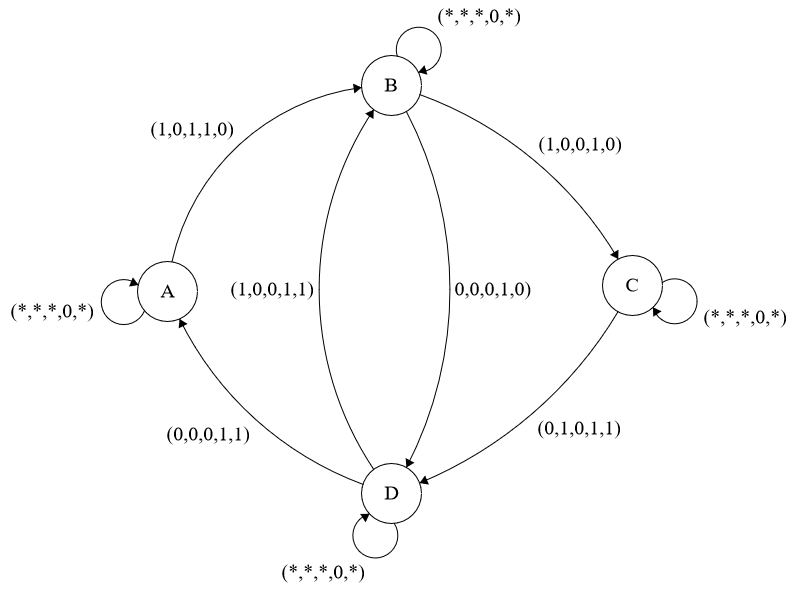
\includegraphics[width=1\textwidth]{img/maquina/maquinaEstado}
			 \caption*{Nota: A entrada está está no formato ( b, a, f, m, s ). Os
			  significados dos estados estão no \autoref{quadro:significadoEstados}.}
		\end{figure}

		\begin{quadro}[H]
			\centering
			\caption{Significados dos estados relacionando com os estados reais do problema proposto.}
			\label{quadro:significadoEstados}
			\begin{tabular}{|c|l|}
			  \hline
			   \textbf{Estado} & \textbf{Significado}\\
			    \hline
				   A & Totalmente fechado \\
			   	\hline
			   		B & Abrindo \\
			    \hline
					C & Totalmente aberto \\
			    \hline
			    	D & Fechando \\
			    \hline
			\end{tabular}
			\legend{Fonte: Próprio Autor}
		\end{quadro}

	\section{Passo 2 - Escrever um código Verilog para a máquina de estado}
		Para a realização deste passo, foram utilizados o programa Quartus 13.0 SP 1
		 e a placa \ac{fpga} Cyclone II - EP2C20F484C7.

		Com a máquina de estado pronto, criou-se a código em Verilog, que no
		estado\ "totalmente aberto"\ apresenta A \textit{display}, no estado\ "totalmente fechado"\
		apresenta F no \textit{display}, no estado\ "abrindo"\ acende um \ac{led} verde e no
		estado "fechando"\ acente um \ac{led} vermelho. Nos estados "abrindo"\ e "fechando"\ o
		\textit{display} apresenta 0. O Verilog encontra-se no \autoref{codigo:maquina} e o resultado da
		compilação na \autoref{figura:compilacaoMaquina}.

		\lstinputlisting[label = {codigo:maquina},caption = {Código da máquina de estado do problema da garagem.}]
		{codigo/maquina.v}

		\begin{figure}[H]
			 \centering
			 \caption{\label{figura:compilacaoMaquina}Resultado da compilação do código da máquina de
			  estado do problema da garagem.}
			 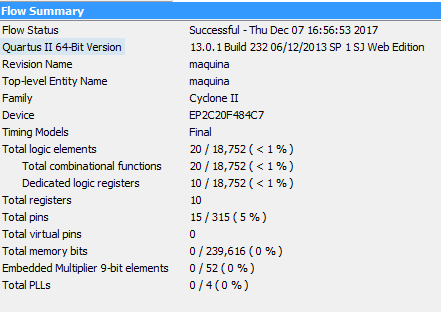
\includegraphics[width=1\textwidth]{img/maquina/compilacao}
		\end{figure}

		Para a realização dos testes, criou-se um \textit{test bench} conforme o \autoref{codigo:testBenchMaquina}.
		Além disto, fez-se o \textit{deploy} na \ac{fpga}\footnote{Os resultados dos
		 testes e simulações encontram-se na Avaliação dos resultados.}.

		\lstinputlisting[label = {codigo:testBenchMaquina},caption = {Código de \textit{test bench} da máquina do problema da garagem.}]
		{codigo/maquina_TB.v}





%Apresentar   o   detalhamento   da  execução  e   resultados   dos   passos   realizados
%durante   o   experimento,   incluindo   tabelas   verdade,   esquemáticos,   e   código
%(quando  houver).
%Especificar  componentes,  sistemas  e  instrumentos  utilizados.
%Usar listas, figuras e quadros, descrevê-los e discuti-los.
